In this section, we are going to investigate the numerical methods for computing the Casimir energy. 
We would like to use the following notations for the domains of the boundary integral operators in both scalar and vector case. Assume 
$\Omega^{-}\in\mathbb{R}^{d}$, for $d \geq 2$ is the interior bounded Lebesgue-measurable domain that the scatterer occupies with Lipschitz-continuous boundary $\Gamma$ and 
$\Gamma:=\partial\Omega$ has a finite number of smooth faces that meet at non-degenerate edges and corners. In addition, the exterior domain is denoted as 
$\Omega^{+} = \mathbb{R}^{d}\backslash\overline{\Omega^{-}}$. $\boldsymbol{n}$ is the exterior unit normal to the surface $\Gamma$ pointing outwards from $\Omega^{-}$ and 
$\boldsymbol{n}_{\boldsymbol{x}}$ is normal to $\Gamma$ at the point $\boldsymbol{x}\in\Gamma$.

In the scalar case, the Casimir energy can be expressed in terms of the single-layer boundary operator and we will start from defining the function space 
on which the boundary operators are well-defined and Dirichlet trace operator, then give the definition of the single-layer boundary operator. Afterwards, the relation between the Krein 
spectral shift function with this operator will be introduced and finally, the numerical framework for computing the Casimir energy in the scalar case 
via the Galerkin discretization of the single-layer boundary operator.
\subsection{Scalar function space and trace operator}
For the bounded interior domain $\Omega^{\pm}$ or the unbounded exterior domain $\Omega^{+}$, the space of the square integrable functions is 
\begin{align*}
    L^{2}(\Omega^{\pm}) := \left\{f:\Omega^{\pm}\rightarrow\mathbb{C}, f \text{ is Lebesgue measurable and} \int_{\Omega^{\pm}}|f|^{2} < \infty \right\}
\end{align*}
and the Sobolev space $H^{s}(\Omega^{\pm})$ is defined as 
\begin{align*}
    H^{s}(\Omega^{\pm}):=\left\{f\in L^{2}(\Omega^{\pm}), \forall\alpha \text{ s.t.} |\alpha|\leq s, D^{\alpha}f\in L^{2}(\Omega^{\pm})\right\},
\end{align*}
where $\alpha = (\alpha_{1}, \alpha_{2}, \dots, \alpha_{d})$ is a multi-index and $|\alpha| = \alpha_{1} + \alpha_{2} + \dots + \alpha_{d}$, and 
the derivative is defined in the weak sense.

To construct the single-layer boundary operator, we also need the Dirichlet trace operator 
$\gamma_{\text{D}}^{\pm}: H^{1}(\Omega^{\pm})\rightarrow H^{\frac{1}{2}}(\Gamma)$: for sufficiently smooth function $p$,
\begin{align*}
    \gamma_{\text{D}}^{\pm}p(\boldsymbol{x}):=\lim_{\Omega^{\pm}\ni\boldsymbol{x'}\rightarrow\boldsymbol{x}\in\Gamma}p(\boldsymbol{x'}),
\end{align*}
where the subscripts $^{-}$ and $^{+}$ denote the interior and exterior traces, respectively. 

\subsection{Single-layer boundary integral operator}%==========================================================================================
Typically, the \emph{single-layer potential operator} $\mathcal{V}_{k}: H^{-\frac{1}{2}}(\Gamma)\rightarrow H^{1}(\Omega^{\pm})$ can be represented as 
\begin{align*}
    (\mathcal{V}_{k}\mu)(\boldsymbol{x}) := \int_{\Gamma}g_{k}(\boldsymbol{x},\boldsymbol{y})\psi(\boldsymbol{y})dS_{\boldsymbol{y}}, \ \ \ \ \ 
    \text{for}\ \mu\in H^{-\frac{1}{2}}(\Gamma) \  \text{and} \ \boldsymbol{x}\in\Omega^{\pm}\backslash\Gamma,
\end{align*}
where $g_{k}(\boldsymbol{x},\boldsymbol{y})$ is the fundamental solution of the Helmholtz operator and especially,
\begin{align}\label{Green's function}
    g_{k}(\boldsymbol{x},\boldsymbol{y}) = \begin{cases}
          \frac{\mathrm{i}}{4}H_{0}^{(1)}(k|\boldsymbol{x}-\boldsymbol{y}|), \ \ \ \ &\text{for} \ d = 2\\
          \frac{e^{ik|\boldsymbol{x}-\boldsymbol{y}|}}{4\pi|\boldsymbol{x} - \boldsymbol{y}|}, \ \ \ \ &\text{for} \ d = 3,
        \end{cases}
\end{align}
where $H_{0}^{(1)}$ is a Hankel function of the first kind.

Now we can derive the \emph{single-layer boundary operator}
$V_{k}: H^{-\frac{1}{2}}(\Gamma)\rightarrow H^{\frac{1}{2}}(\Gamma)$ from this potential operator:
\begin{align*}
    (V_{k}\mu)(\boldsymbol{x}) := \{\gamma_{\text{D}}\mathcal{V}_{k}\mu\}_{\Gamma}(\boldsymbol{x}).
\end{align*}
Combining with the jump condition
\begin{align*}
    [\gamma_{\text{D}}]_{\Gamma}\mathcal{V}_{k} = \gamma_{\text{D}}^{+}\mathcal{V}_{k} - \gamma_{\text{D}}^{+}\mathcal{V}_{k} = 0, 
\end{align*}
we can derive that 
\begin{align*}
    \gamma_{\text{D}}^{+}\mathcal{V}_{k} = \gamma_{\text{D}}^{-}\mathcal{V}_{k} = V_{k},
\end{align*}
for the exterior and interior traces and the single-layer boundary operator writes 
\begin{align*}
    (V_{k}\mu)(\boldsymbol{x}) := \int_{\Gamma}g_{k}(\boldsymbol{x},\boldsymbol{y})\psi(\boldsymbol{y})dS_{\boldsymbol{y}}, \ \ \ \ \ 
    \text{for}\ \mu\in H^{-\frac{1}{2}}(\Gamma) \  \text{and} \ \boldsymbol{x}\in\Gamma.
\end{align*}
\subsection{Relation between the Krein spectral shift function and the single-layer boundary operator}
By \cite{hanisch2020relative}, the Krein spectral shift function is defined as 
\begin{align*}
    \xi(k) = \frac{1}{2\pi \mathrm{i}}\log\left(\frac{\det(S(k))}{\det(S_{1,k})\cdots\det(S_{N,k})}\right),
\end{align*}
where $S_{i,n}$ is the scattering matrix associated with the $n$th scatterer. These scattering matrices can be constructed  $S_{i,n} = I + T_{i,n}$, where 
$I$ is the identity matrix and $T_{i,n}$ is the $T$-matrix and the method of computing the $T$-matrix is fully discussed in \cite{waterman1969new} and 
\cite{ganesh2008far}.

The following theorem links the single-layer boundary operator with the Krein spectral shift function which inspires us to computing the Casimir energy 
via the scattering matrix or integral operator. 
\begin{theorem}\cite{hanisch2020relative}
    Consider $\Omega$ as a domain assembling from individual objects $\Omega_{i}$. Let $V_{k}$ be the single-layer boundary operator defined on the boundary 
    $\partial\Omega = \bigcup_{i = 1}^{N}\partial\Omega_{i}$, and $\tilde{V}_{k}$ is the ``diagonal part'' of $V_{k}$ by restricting the integral 
    kernel to the subset $\bigcup_{i = 1}^{N}\partial\Omega_{i}\times\partial\Omega_{i}\subset\partial\Omega\times\partial\Omega$ then the operator 
    $V_{k}\tilde{V}_{k}^{-1}$ is trace-class and 
    \begin{align*}
        \Xi(k) = \log\det\left(V_{k}\tilde{V}_{k}^{-1}\right).
    \end{align*}

    Then for $k >0$, we have 
    \begin{align*}
        -\frac{1}{\pi}\emph{\text{Im}}\Xi(k) = \frac{\mathrm{i}}{2\pi}(\Xi(k) - \Xi(-k)) = \xi(k)
    \end{align*}
    and by choosing $f(x) = x$ in \eqref{B-K formula}, this gives the formula 
    \begin{align}\label{slp and matrix}
        \emph{\text{Tr}}\left(\Delta^{\frac{1}{2}} + (N - 1)\Delta_{0}^{\frac{1}{2}} - \sum_{i = 1}^{N}\Delta_{j}^{\frac{1}{2}}\right)  = 
        \int_{0}^{\infty}\xi(k)dk = -\frac{1}{\pi}\int_{0}^{\infty}\Xi(\mathrm{i}k)dk.
    \end{align}
\end{theorem}

The equation \eqref{slp and matrix} is used to compute the Casimir energy between the objects and the formula is written as
\begin{align}\label{KSSF and CasE}
    \mathcal{E} = \frac{\hbar c}{2}\int_{0}^{\infty}\xi(k)dk = -\frac{\hbar c}{2\pi}\int_{0}^{\infty}\Xi(\mathrm{i}k)dk
\end{align}

\begin{remark}
    Note that the integral $\frac{\hbar c}{2}\int_{0}^{\infty}\xi(k)dk$ in \eqref{KSSF and CasE} is not Lebesgue convergence but might be Riemann integrable. 
    Therefore, one should compute Casimir energy via the integral operator method but not the scattering matrix method.
\end{remark}
\subsection{Galerkin discretization and boundary element spaces}
In order to compute the integral \eqref{KSSF and CasE}, we need to compute the log determinant of the operators $V_{k}\tilde{V}_{k}^{-1}$. In our numerical 
framework, we would like to use the Galerkin discretization to express the operators in matrix form and in this part, the explicit form of the element inside
the matrix will be given and the Corresponding basis functions will be introduced as well.

Recall the domain of the single-layer boundary operator is $H^{-\frac{1}{2}}(\Gamma)$. To discretize this Sobolev space, we would lke to introduce the 
triangulation $\mathcal{T}_{h}$ of the boundary surface $\Gamma$ with triangular surface elements $\tau_{l}$ and associated nodes $\boldsymbol{x}_{i}$ 
s.t. $\overline{\mathcal{T}_{h}} = \bigcup_{l}\overline{\tau_{l}}$, where $h$ is the mesh size and define the space of the continuous piecewise linear functions
\begin{align*}
    P_{h}^{1}(\Gamma) = \{v_{h}\in C^{0}(\Gamma): v_{h}|_{\tau_{l}}\in\mathbb{P}_{1}(\tau_{l}), \ \text{for} \ \ \tau_{l}\in\mathcal{T}_{h}\},
\end{align*}
where $\mathbb{P}_{1}(\tau_{l})$ denotes the space of polynomials of order less than or equal to 1 on $\tau_{1}$
and typically, we use the following $P_{h}^{1}(\Gamma)$ space to discretize $H^{-\frac{1}{2}}(\Gamma)$:
\begin{align*}
    P_{h}^{1}(\Gamma) := \text{span}\{\phi_{j}\} \subset H^{-\frac{1}{2}}(\Gamma)
\end{align*}
with 
\begin{align*}
    \phi_{j}(\boldsymbol{x}_{i}) = \begin{cases}
        1, & i = j,\\
        0, & i\neq j.
    \end{cases}
\end{align*}

Having defined the basis function $P_{h}^{1}(\Gamma)$, we can represent each element inside the Galerkin discretization form. Assume there are $N$ objects,
then the matrix of the operator $V_{k}$ is an $N$ by $N$ block matrix, written as 
\begin{align}\label{matrix V}
    \mathsf{V}_{k} = \mathsf{V}(k) = \begin{bmatrix}
        \mathsf{V}_{11}(k) & \mathsf{V}_{12}(k) & \cdots & \mathsf{V}_{1N}(k) \\
        \mathsf{V}_{21}(k) & \mathsf{V}_{22}(k) & \cdots & \mathsf{V}_{2N}(k) \\
        \vdots & \vdots & \ddots & \vdots \\
        \mathsf{V}_{N1}(k) & \mathsf{V}_{N2}(k) & \cdots & \mathsf{V}_{NN}(k) \\
\end{bmatrix}
\end{align}
and the matrix $\tilde{V}_{k}$ is the diagonal part of $V_{k}$:
\begin{align}\label{matrix tilde V}
    \tilde{\mathsf{V}}_{k} =  \tilde{\mathsf{V}}(k) = \begin{bmatrix}
        \mathsf{V}_{11}(k) & 0      & \cdots & 0 \\
    0      & \mathsf{V}_{22}(k) & \cdots & 0\\
    \vdots & \vdots & \ddots & \vdots \\
    0      & 0      & \cdots & \mathsf{V}_{NN}(k) \\
\end{bmatrix}.
\end{align}
Therefore, the element in the $m$th row and $n$th column of the block matrix $\mathsf{V}_{ij}(k)$ is 
\begin{align}\label{Elements in matrix V}
    \mathsf{V}_{ij}^{(m,n)} (k) = \langle V_{ij}(k)\phi_{m}^{(i)}, \phi_{n}^{(j)}\rangle = 
    \int_{\Gamma}\overline{\phi_{n}^{(j)}}(\boldsymbol{x})\int_{\Gamma}g_{k}(\boldsymbol{x}, \boldsymbol{y})\phi_{m}^{(i)}(\boldsymbol{y})dS_{\boldsymbol{y}}dS_{\boldsymbol{x}},
\end{align}
where $\boldsymbol{\phi}^{(i)} = \begin{bmatrix}
    \phi_{1}^{(i)} & \phi_{2}^{(i)} & \dots & \phi_{N}^{(i)}
\end{bmatrix}$ is the set of basis functions defined on the $i$th object and 
\begin{align*}
    \langle f, g \rangle = \int_{\Gamma}\overline{f(\boldsymbol{x})}g(\boldsymbol{x})dS_{x}
\end{align*}
denotes the standard $L^{2}(\Gamma)$ inner product.


By \eqref{Elements in matrix V}, the explicit form of each element in matrix $\mathsf{V}_{k}$ and $\tilde{\mathsf{V}}_{k}$ is known, therefore,
the value of $\Xi(\mathrm{i}k)$ = $\log\det(V_{\mathrm{i}k}\tilde{V}_{\mathrm{i}k}^{-1})$ can be evaluated by computing 
$\log\frac{\det\mathsf{V}_{\mathrm{i}k}}{\det\tilde{\mathsf{V}}_{\mathrm{i}k}}$ with 
different values of $k$, which is the integrand of the Casimir formula \eqref{KSSF and CasE}. However, by plotting the value of this integrand 
with respect to different values of $\mathrm{i}k$, we found that this function is exponentially decays with increasing the imaginary wavenumber 
$\mathrm{i}k$ (see Figure \ref{The integrand decays exponentially} (Left)) and shares the same trend with $e^{-2Zk}$,  where $Z$ is the minimal distance 
between two objects. This result is proved and summarized in the following theorem. 


\begin{theorem}
    Let $\mathsf{V}_{\mathrm{i}k}$ and $\tilde{\mathsf{V}}_{\mathrm{i}k}$ be the positive definite block matrices defined in \eqref{matrix V} and \eqref{matrix tilde V} 
    and they are partitioned as 
    2 by 2 block matrices
    \begin{align*}
        \mathsf{V}_{\mathrm{i}k} = \begin{bmatrix}
            \mathbb{V}_{11}(\mathrm{i}k) & \mathbb{V}_{12}(\mathrm{i}k)\\
            \mathbb{V}_{21}(\mathrm{i}k) & \mathbb{V}_{22}(\mathrm{i}k)
        \end{bmatrix} \ \ \text{and} \ \   \tilde{\mathsf{V}}_{\mathrm{i}k} = \begin{bmatrix}
            \mathbb{V}_{11}(\mathrm{i}k) & 0\\
            0 & \mathbb{V}_{22}(\mathrm{i}k)
        \end{bmatrix}.
    \end{align*} Denote 
    $\{\lambda_{i}\}_{i}$ and $\{\tilde{\lambda}_{i}\}_{i}$ as the eigenvalues of them, separately and $Z$ be the minimal distance between the objects.
    Then, \begin{align*}
        ||\mathsf{V}_{\mathrm{i}k} - \tilde{\mathsf{V}}_{\mathrm{i}k}||_{2} = \mathcal{O}(e^{-Zk})
    \end{align*}
    and the integrand in \eqref{KSSF and CasE} satisfies
    \begin{align}\label{logdet trend}
        \log\frac{\det\mathsf{V}_{\mathrm{i}k}}{\det\tilde{\mathsf{V}}_{\mathrm{i}k}} = \frac{\mathcal{O}(e^{-2Zk})}{\tilde{\lambda}_{\emph{min}}\emph{gap}_{\emph{min}}},
    \end{align}
    where $\tilde{\lambda}_{\emph{min}} = \emph{min}_{i}\tilde{\lambda}_{i}$ and $\emph{gap}_{\emph{min}} = \emph{min}_{i}\emph{gap}_{i}$ with $\emph{gap}_{i}$ defined as 
    \begin{align*}
        \emph{gap}_{i}:= \begin{cases}
            \emph{min}_{\tilde{\lambda}_{j}\in\mathbb{V}_{22}}|\tilde{\lambda_{i}} - \tilde{\lambda_{j}}|, \ \ \emph{if}\ \ \tilde{\lambda}_{i} \in \lambda(\mathbb{V}_{11})\\
            \emph{min}_{\tilde{\lambda}_{j}\in\mathbb{V}_{11}}|\tilde{\lambda_{i}} - \tilde{\lambda_{j}}|, \ \ \emph{if}\ \  \tilde{\lambda}_{i} \in \lambda(\mathbb{V}_{22}).
        \end{cases}
    \end{align*} 
\end{theorem}
\begin{proof}
    By setting $E_{\mathrm{i}k} = \mathsf{V}_{\mathrm{i}k} - \tilde{\mathsf{V}}_{\mathrm{i}k}$, we have 
    \begin{align*}
        ||E_{\mathrm{i}k}||_{2} = \left|\left|\begin{bmatrix}
            0 & \mathbb{V}_{12}(\mathrm{i}k)\\
            \mathbb{V}_{21}(\mathrm{i}k) & 0
        \end{bmatrix}\right|\right|_{2}.
    \end{align*}
    Since the elements in $\mathbb{V}_{12}(\mathrm{i}k)$ and $\mathbb{V}_{21}(\mathrm{i}k)$ are constructed by \eqref{Elements in matrix V} which includes the 
    Green's function $g_{\mathrm{i}k}$ \eqref{Green's function}, we can conclude $||E_{\mathrm{i}k}||_{2} = \mathcal{O}(e^{-Zk})$, where
    $Z$ is the minimal distance between the objects. 

    To prove \eqref{logdet trend}, we firstly assume the eigenvalues of the matrices $\mathsf{V}_{\mathrm{i}k} $ and $\tilde{\mathsf{V}}_{\mathrm{i}k}$
    are  $\{\lambda_{i}\}_{i}$ and $\{\tilde{\lambda}_{i}\}_{i}$, respectively. Then, according to \cite[Theorem 1]{nakatsukasa2015off}, since $E_{\mathrm{i}k}$ and $\tilde{\mathsf{V}}_{\mathrm{i}k}$
    are symmetric matrices, we have the eigenvalue perturbation bound
    \begin{align}\label{gap}
        |\lambda_{i} - \tilde{\lambda}_{i}| \leq \frac{||E_{\mathrm{i}k}||_{2}^{2}}{\text{gap}_{i}},
    \end{align}
    where 
    \begin{align*}
        \text{gap}_{i}:= \begin{cases}
            \text{min}_{\tilde{\lambda}_{j}\in\mathbb{V}_{22}}|\tilde{\lambda_{i}} - \tilde{\lambda_{j}}|, \ \ \text{if}\ \ \tilde{\lambda}_{i} \in \lambda(\mathbb{V}_{11})\\
            \text{min}_{\tilde{\lambda}_{j}\in\mathbb{V}_{11}}|\tilde{\lambda_{i}} - \tilde{\lambda_{j}}|, \ \ \text{if}\ \  \tilde{\lambda}_{i} \in \lambda(\mathbb{V}_{22}).
        \end{cases}
    \end{align*} 
    Since  $||E_{\mathrm{i}k}||_{2} = \mathcal{O}(e^{-Zk})$, \eqref{gap} becomes $\lambda_{i} - \tilde{\lambda}_{i} = \frac{\mathcal{O}(e^{-2Zk})}{\text{gap}_{i}}$.
    By setting $\tilde{\lambda}_{\text{min}} = \text{min}_{i}\tilde{\lambda}_{i}$ and $\text{gap}_{\text{min}} = \text{min}_{i}\text{gap}_{i}$, we have 
    \begin{align*}
        \log\frac{\det\mathsf{V}_{\mathrm{i}k}}{\det\tilde{\mathsf{V}}_{\mathrm{i}k}} &= \sum_{i}\log\frac{\lambda_{i}}{\tilde{\lambda}_{i}}\\
        &= \sum_{i}\log\left[1+\frac{\mathcal{O}(e^{-2Zk})}{\tilde{\lambda}_{i}\text{gap}_{i}}\right]\\
        &= \sum_{i} \frac{\mathcal{O}(e^{-2Zk})}{\tilde{\lambda}_{i}\text{gap}_{i}} + \text{h.o.t}\\
        &\leq \sum_{i}\frac{\mathcal{O}(e^{-2Zk})}{\tilde{\lambda}_{\text{min}}\text{gap}_{\text{min}}} + \text{h.o.t}\\
        &= \frac{\mathcal{O}(e^{-2Zk})}{\tilde{\lambda}_{\text{min}}\text{gap}_{\text{min}}} 
    \end{align*}
\end{proof}
Note that the numerical experiments indicate that the eigenvalues $\{\tilde{\lambda}_{i}\}_{i}$ and the eigenvalue gaps $\{\text{gap}_{i}\}_{i}$ do not exponentially
depend on $k$.


\begin{figure}[H]
    \centering
    \hspace*{-1cm}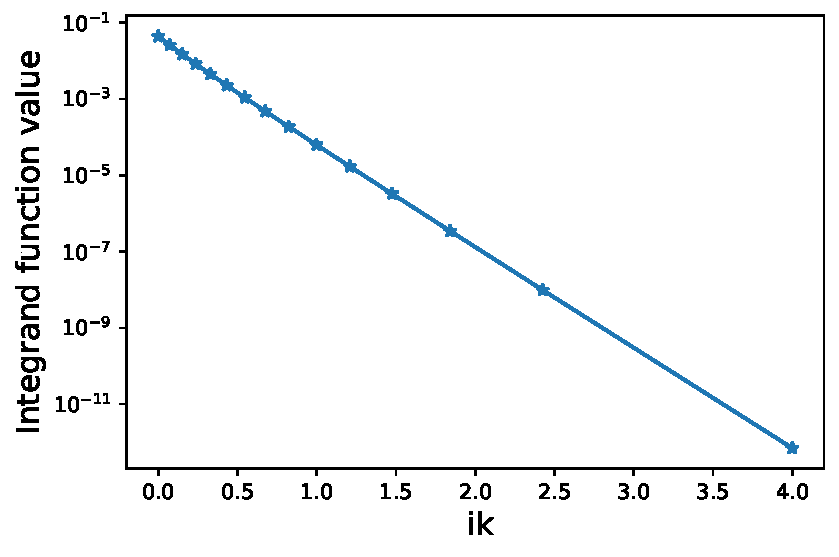
\includegraphics[scale = 0.4]{figures/integ_exp_decay.pdf}
    \caption{(Left) The integrand of the Casimir energy whose value exponentially decays with increasing imaginary wavenumber $\mathrm{i}k$. The integrand function 
    shares the same trend with $e^{-2Zk}$, where $Z$ is the minimal distance between two objects. The scatterers are two spheres with equal radii 
    $R = 1$ with minimal distance $Z = 1.5$. (Right) The integrand of the Casimir energy after changing the 
    variable for applying the trapezoid quadrature rule.}
    \label{The integrand decays exponentially}
\end{figure}


Finally, one can apply the normal trapezoidal rule to calculate the integral 
$\int_{0}^{\infty}\Xi(\mathrm{i}k)dk = \int_{0}^{\infty}\log\frac{\det\mathsf{V}_{\mathrm{i}k}}{\det\tilde{V}_{\mathrm{i}k}}dk$ with variable changed. 
The steps are sketched as follows.

\begin{itemize}
    \item Set $f(k) = \log\frac{\det\mathsf{V}_{\mathrm{i}k}}{\det\tilde{\mathsf{V}}_{\mathrm{i}k}}$ and the range of $k$ is from 0 to $\infty$.
    \item Let $k = -\log(y)$, then the integral $\int_{0}^{\infty}\log\frac{\det\mathsf{V}_{\mathrm{i}k}}{\det\tilde{V}_{\mathrm{i}k}}dk$ becomes 
    $\int_{0}^{\infty}f(k)dk = \int_{0}^{1}\frac{f(-\text{log}(y))}{y}dy$.
    \item Set the range of $k$ as $(\text{lb}, \text{ub})$ \footnote{``ub'' is short for upperbound and ``lb'' is short for lowerbound.} and the corresponding 
    range for $y$ is $(e^{-\text{ub}}, e^{-\text{lb}})\subset[0,1]$.
    \item Choose $m$ quadrature points from the interval $(e^{-\text{ub}}, e^{-\text{lb}})$ and use the trapezoidal rule to evaluate the integral 
    $\int_{e^{-\text{ub}}}^{e^{-\text{lb}}}\frac{f(-\text{log}(y))}{y}dy$. Figure \ref{The integrand decays exponentially} (Right) plots the integrand with regard to new 
    variable $y$($= e^{-k}$).

\end{itemize}



 

